\documentclass{article}    

\usepackage{graphicx}

\begin(document)

\begin{figure}[!ht]
  \begin{center}
  \begin{tabular}{ccc}
    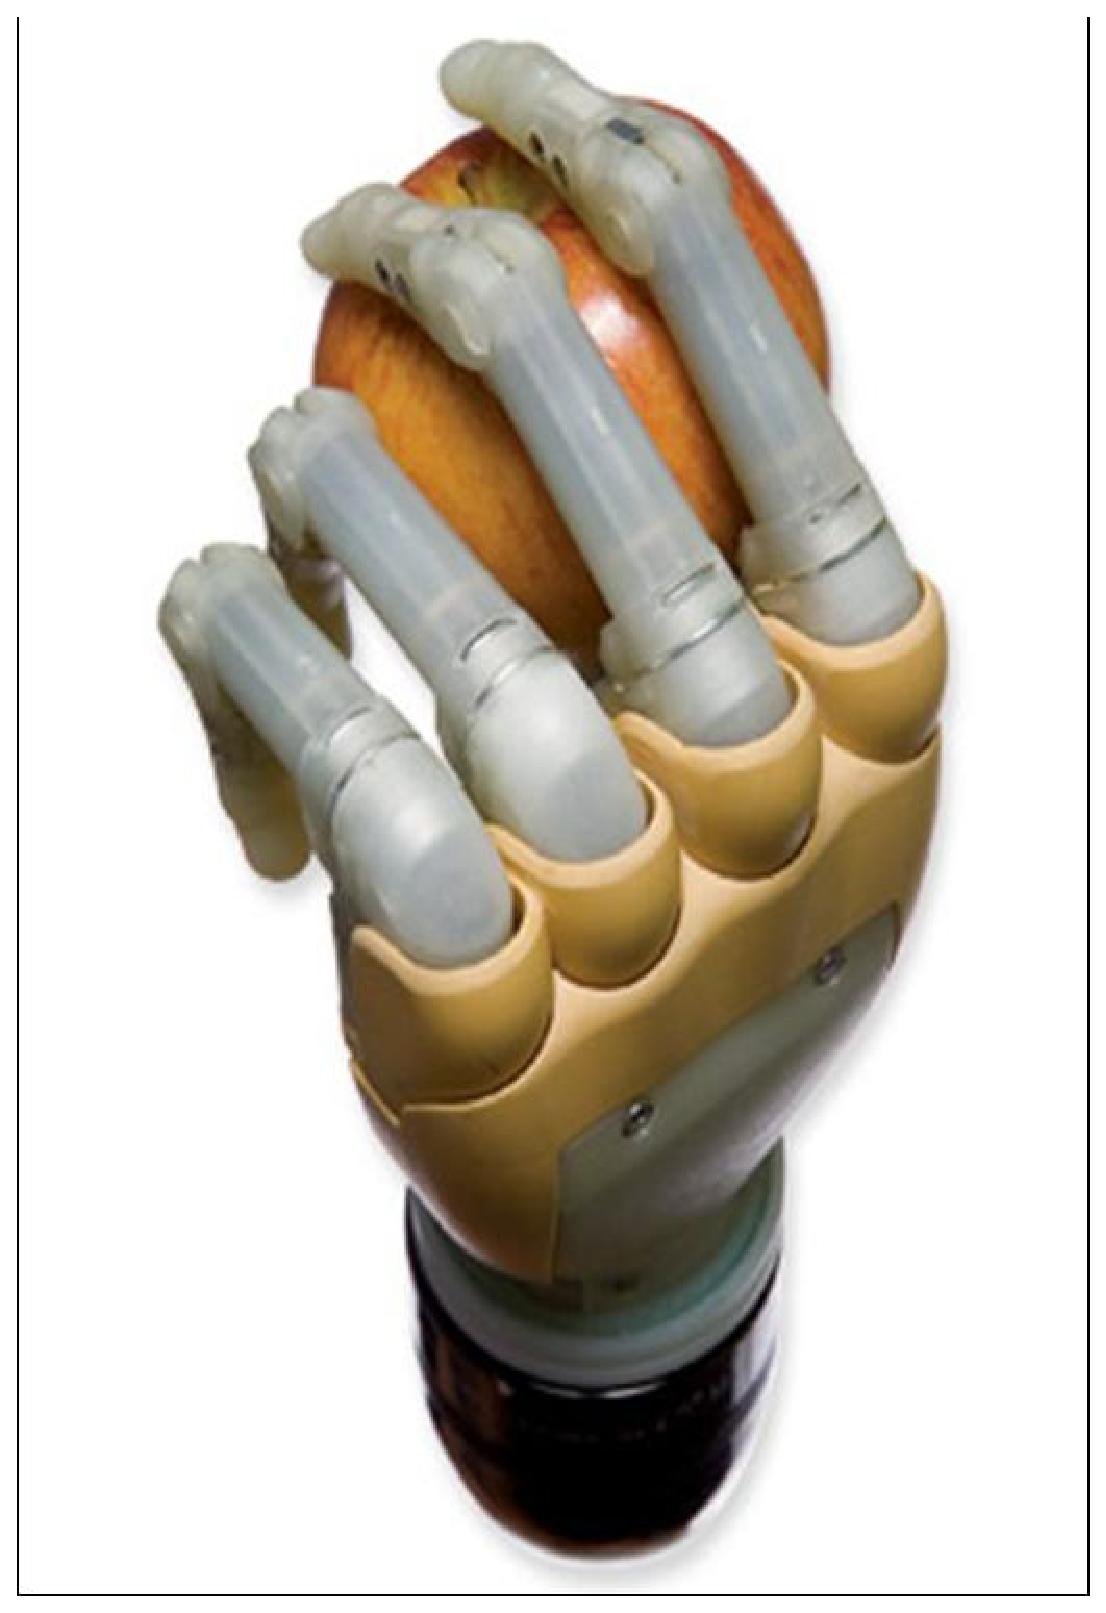
\includegraphics[width=0.25\textwidth]{hands_TB.eps} &
    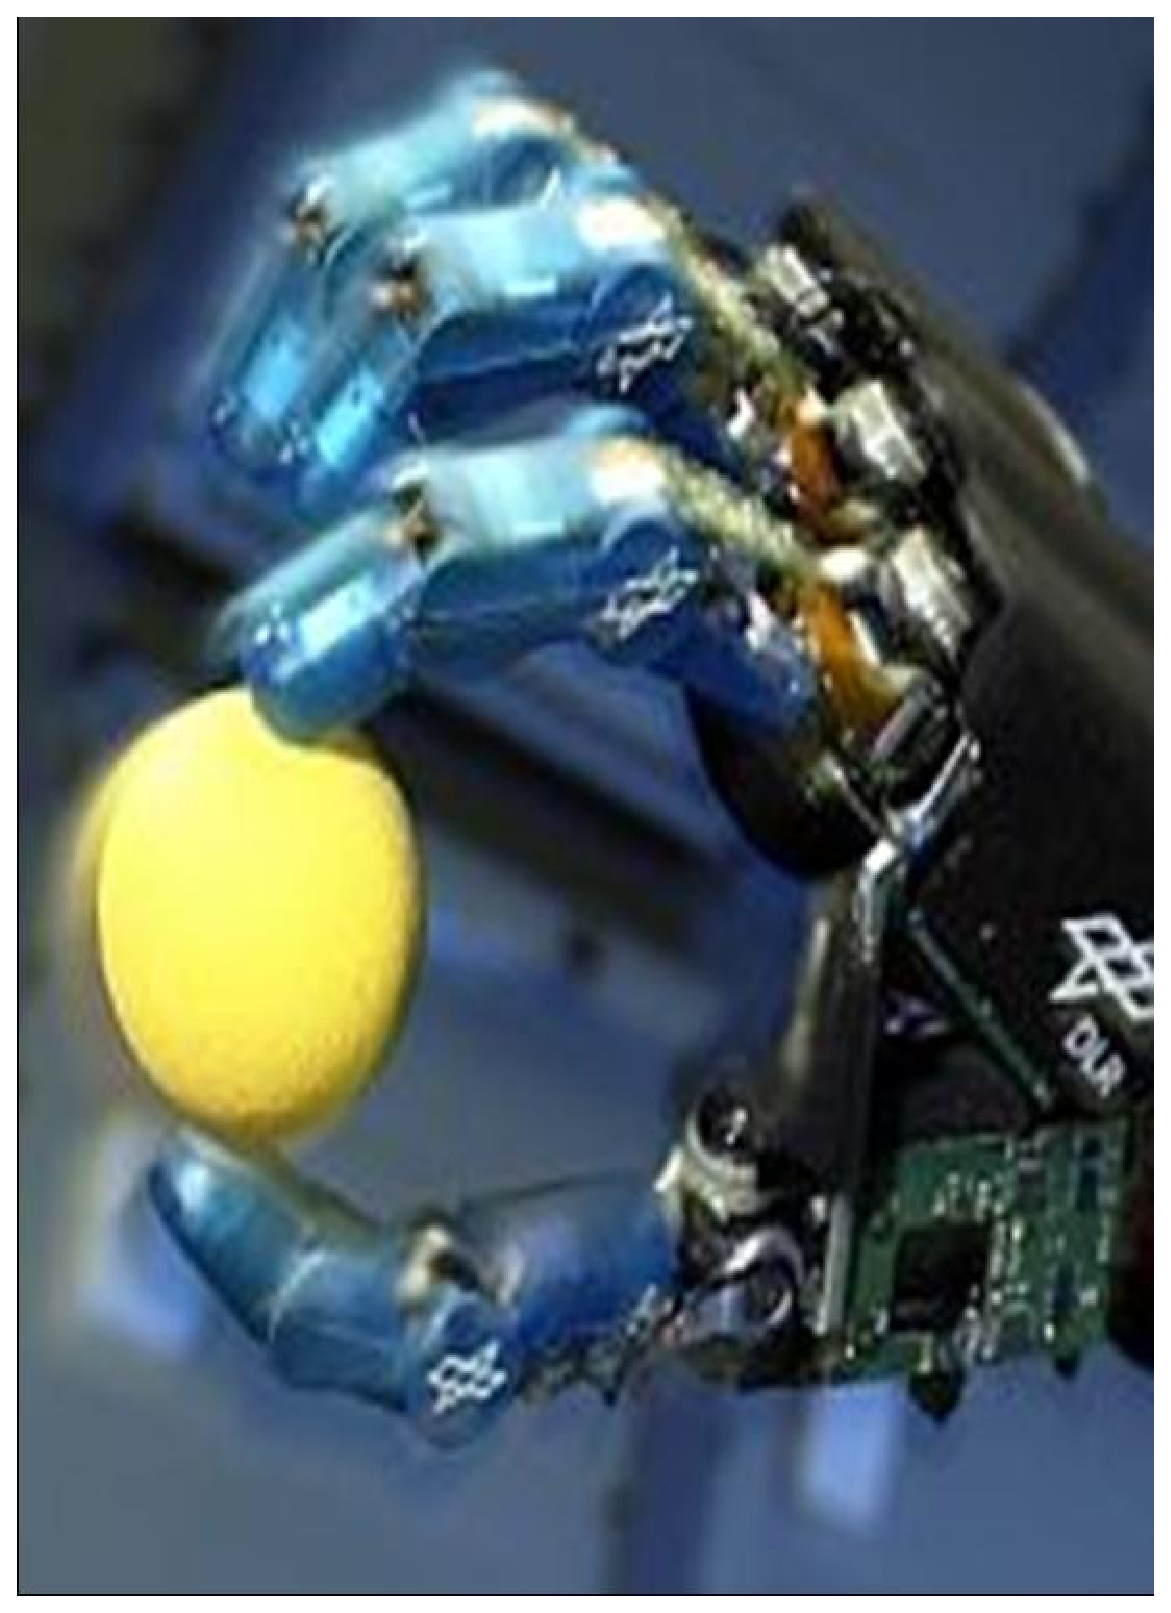
\includegraphics[width=0.25\textwidth]{hands_DLRII.eps} &
    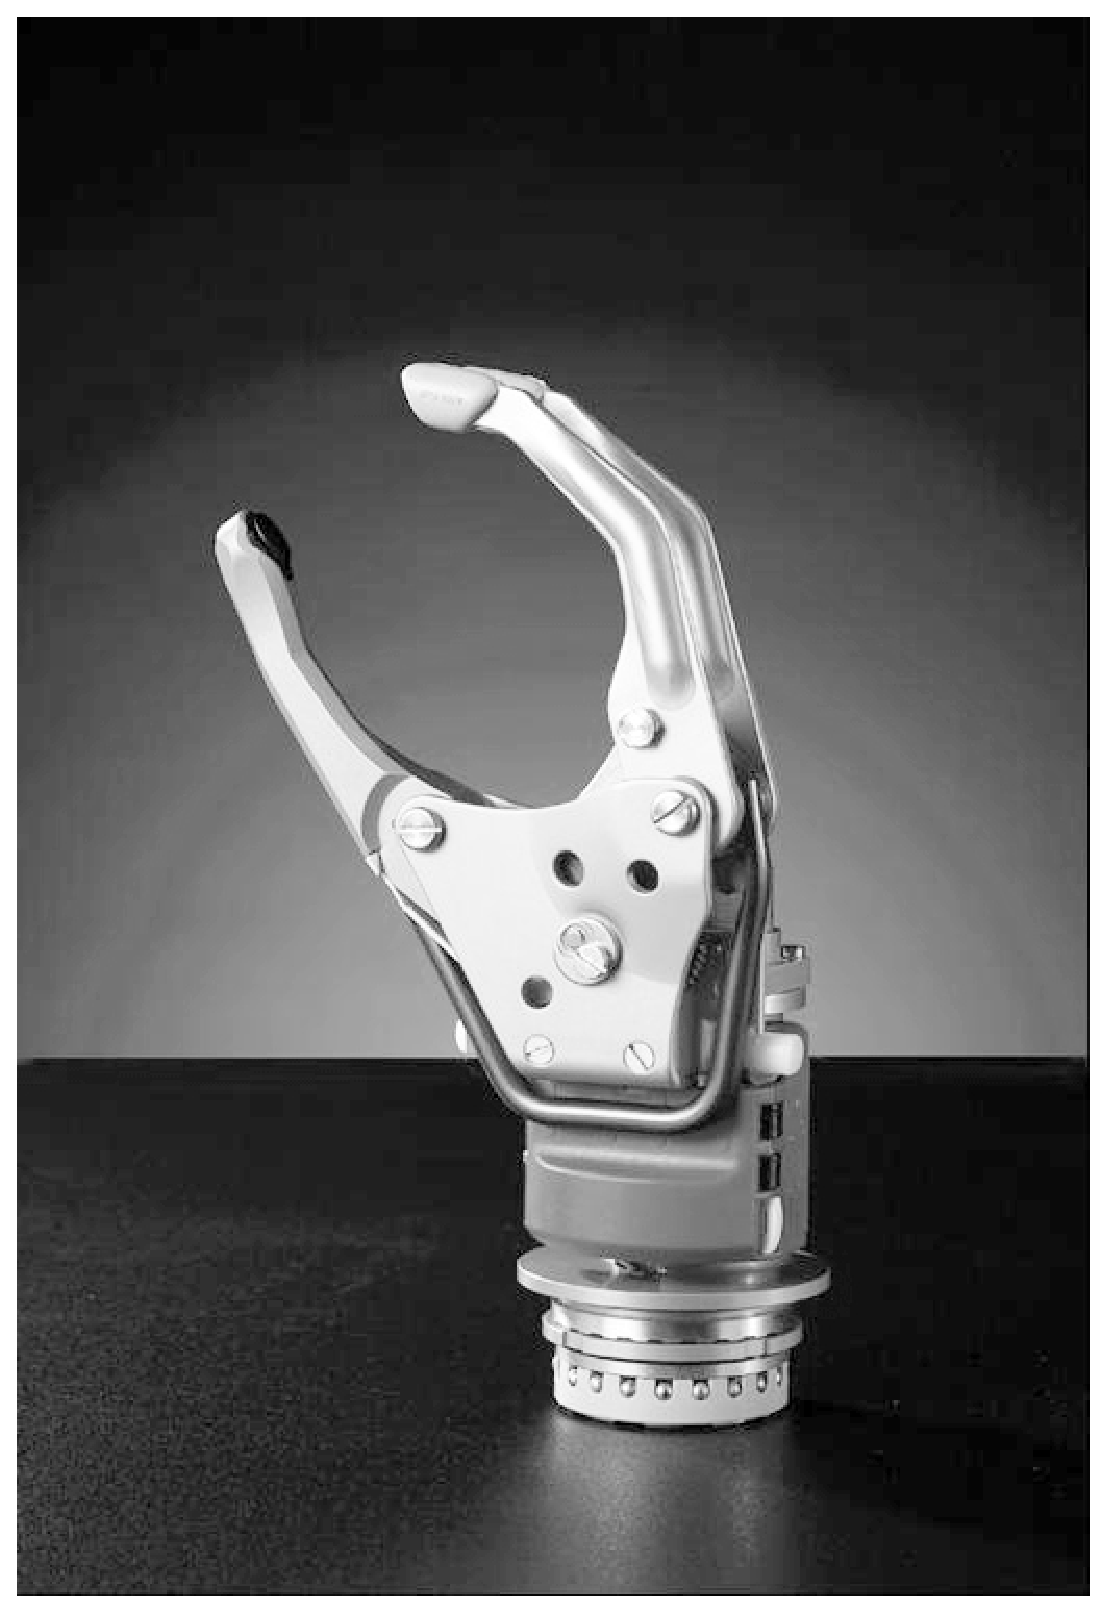
\includegraphics[width=0.25\textwidth]{hands_OB.eps} \\
    $(a)$ & $(b)$ & $(c)$
  \end{tabular}
  \end{center}
%  \caption{$(a)$ Touch Bionics's i-LIMB prosthetic hand (reproduced
%    from \cite{ilimb}); $(b)$ the DLR-II mechanical hand; $(c)$ Otto
%    Bock's SensorHand Speed (reproduced from \cite{sensorhand}).}
%  \label{fig:hands}
\end{figure}

\newpage

\begin{figure}[!ht] \centering
  \begin{tabular}{ccc}
    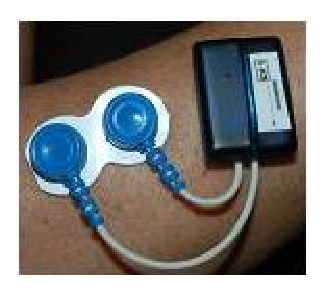
\includegraphics[height=0.16\textheight]{Electrode.eps} &
    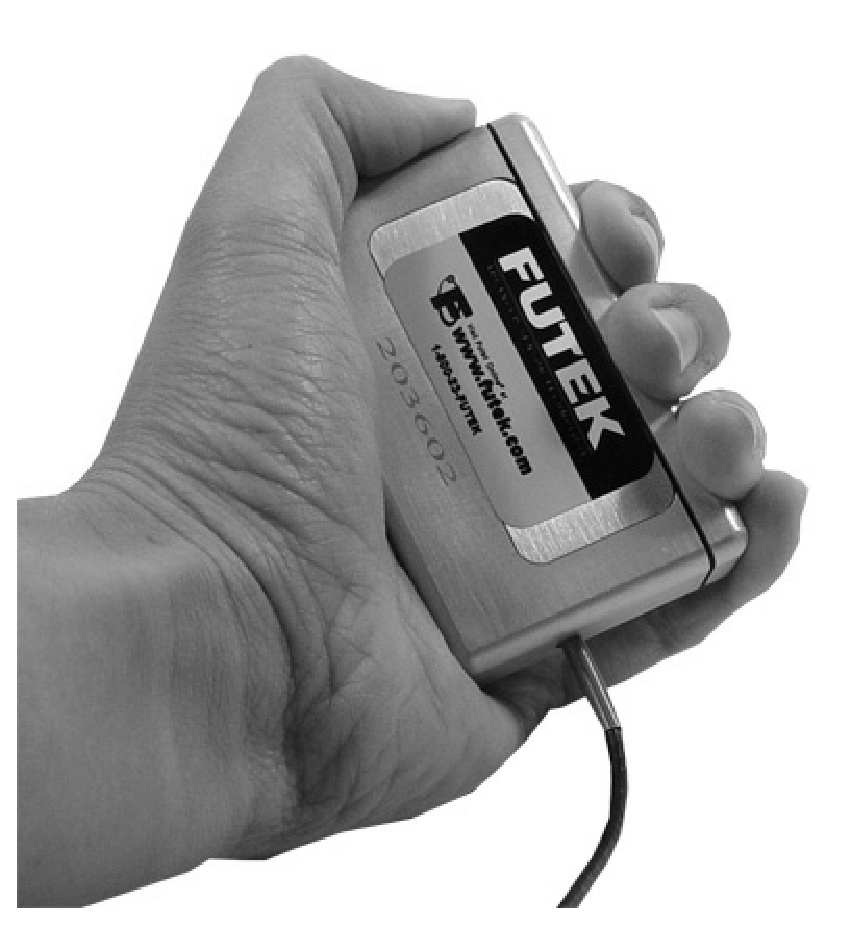
\includegraphics[height=0.16\textheight]{Hand_Gripper.eps} &
    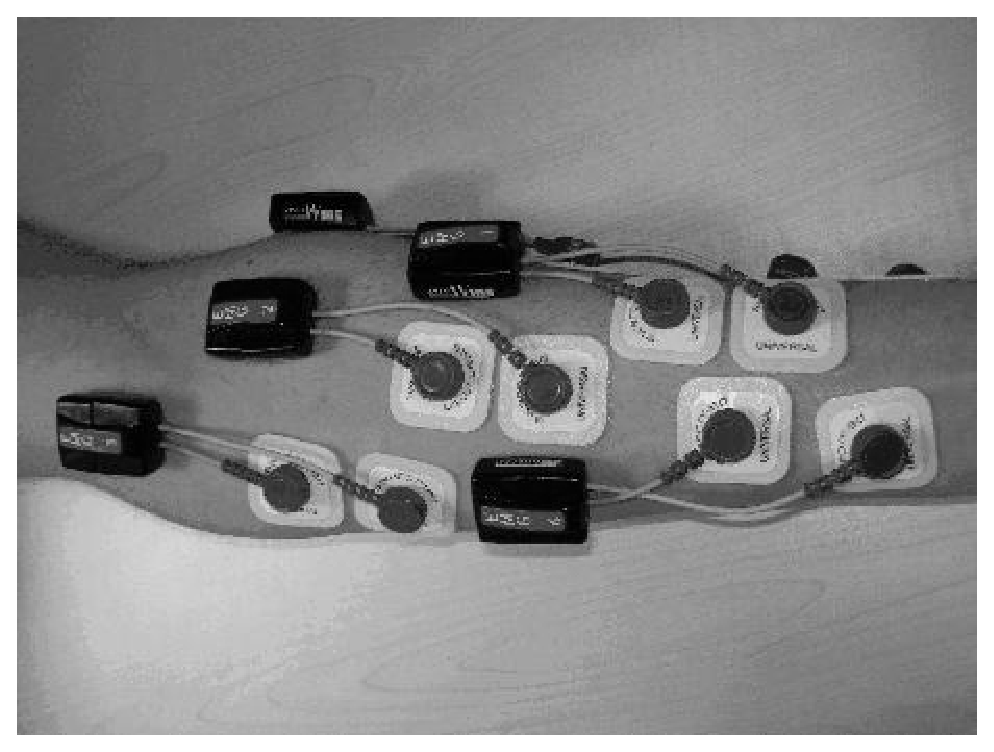
\includegraphics[height=0.16\textheight]{El_Arrangement.eps} \\
    $(a)$ & $(b)$ & $(c)$ \\
  \end{tabular}
%  \caption{The experimental setup (\textit{subject side}): $(a)$ an EMG
%    wireless electrode; $(b)$ the FUTEK force sensor; $(c)$ the typical
%    placement of the EMG electrodes on a subject's forearm (ventral side).}
%  \label{fig:SubjSetup}
\end{figure}

\newpage

\begin{figure}[!ht] \centering
  \begin{tabular}{cc}
    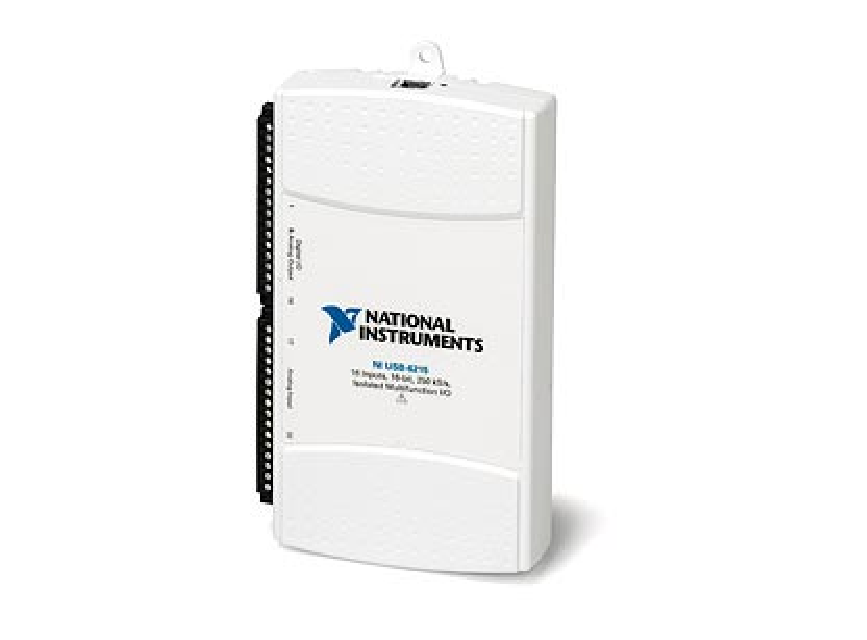
\includegraphics[height=0.16\textheight]{NI-6211.eps} &
    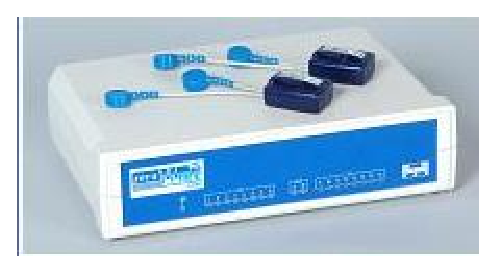
\includegraphics[height=0.16\textheight]{Zero_Base.eps} \\
  $(a)$ & $(b)$\\
  \end{tabular}
%  \caption{The experimental setup (\textit{experimenter side}): $(a)$
%   the USB data acquisition card (NI-USB6211); $(b)$ the EMG device
%   receiver.}
%  \label{fig:ExpSetup}
\end{figure}

\newpage

\begin{figure}[!t] \centering
  \begin{tabular}{ccc}
    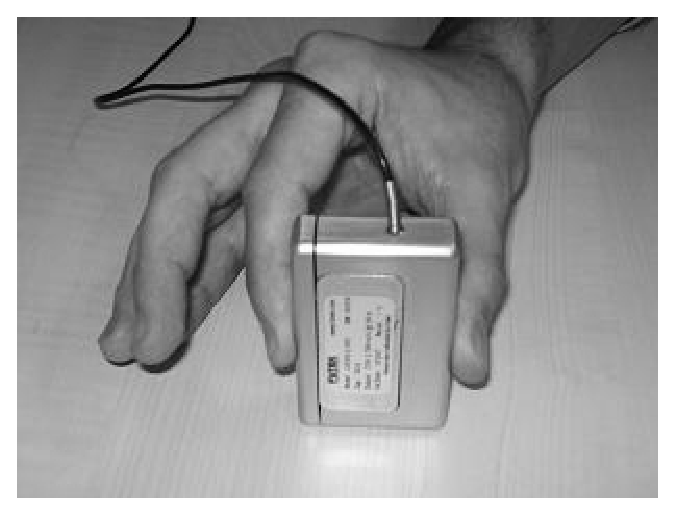
\includegraphics[height=0.16\textheight]{grip1.eps} &
    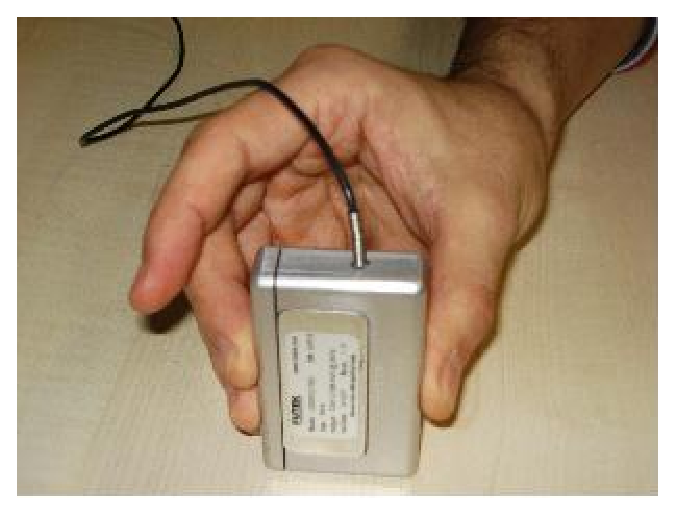
\includegraphics[height=0.16\textheight]{grip2.eps} &
    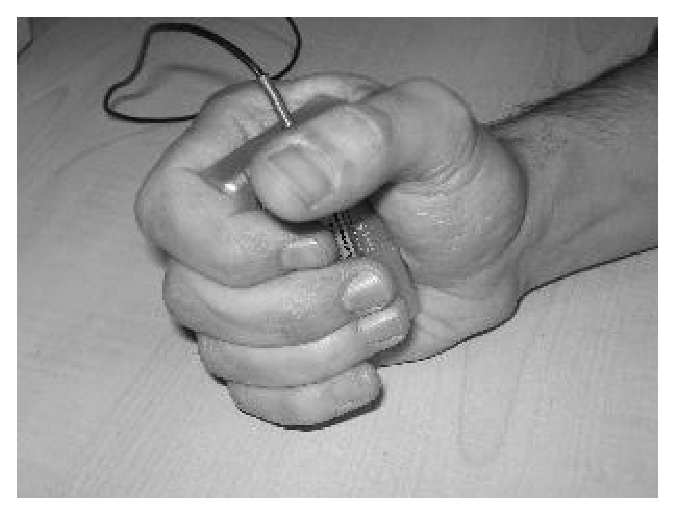
\includegraphics[height=0.16\textheight]{grip3.eps} \\
    $(a)$ & $(b)$ & $(c)$ \\
  \end{tabular}
%  \caption{The three different grips employed in the experiment: $(a)$
%   index precision grip; $(b)$ other fingers precision grip; $(c)$
%   power grasp.}
%  \label{fig:Grasps}
\end{figure}

\newpage

\begin{figure}[!ht] \centering
  \begin{tabular}{cc}
    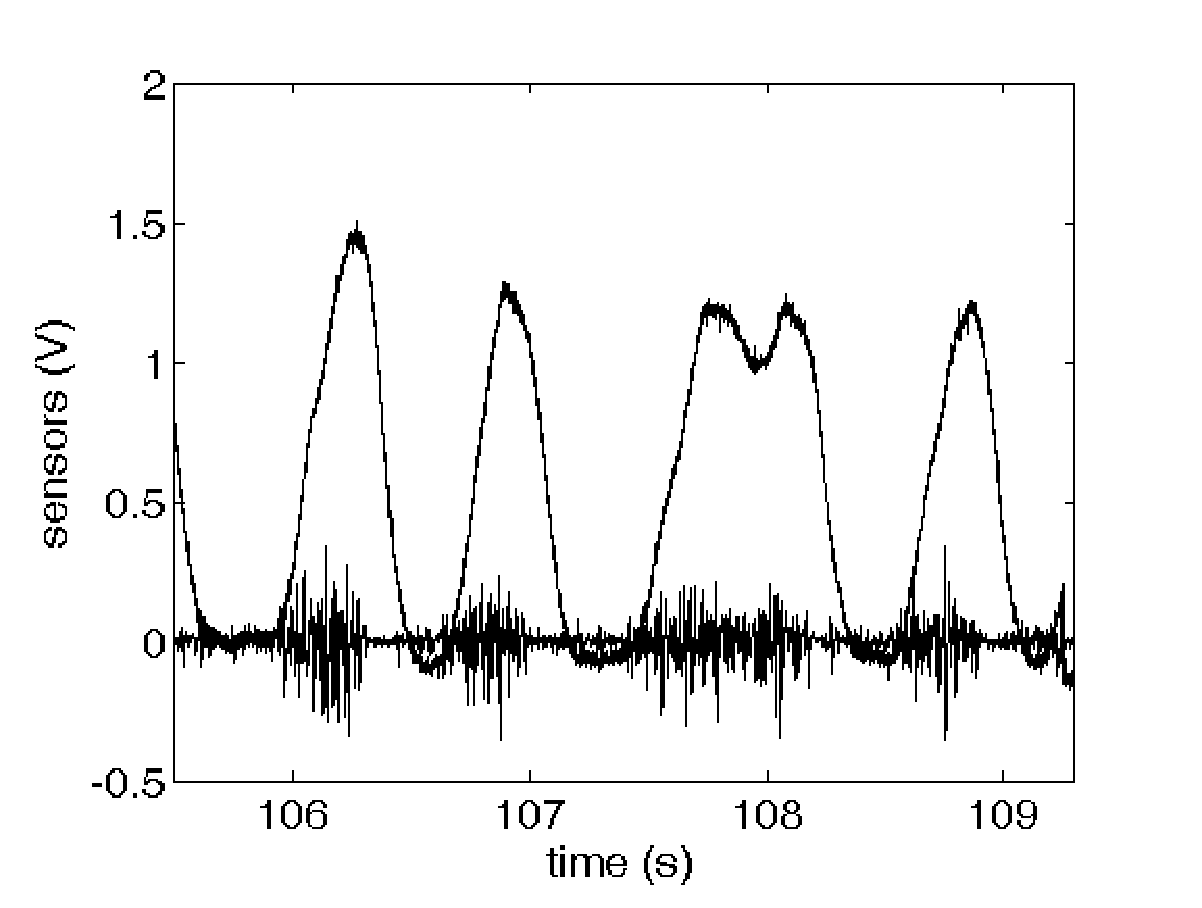
\includegraphics[width=0.45\textwidth]{force_raw.eps} &
    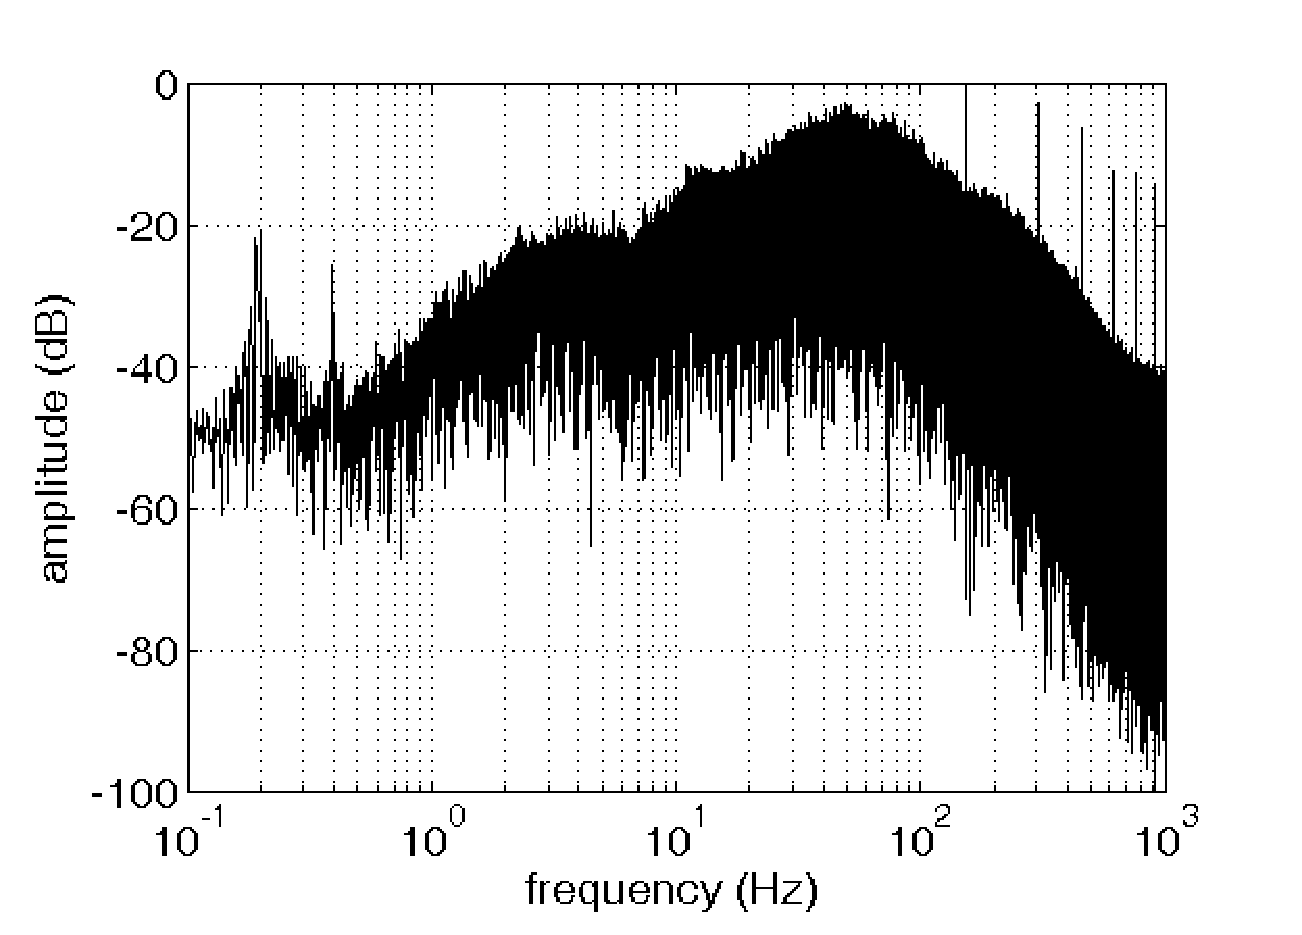
\includegraphics[width=0.45\textwidth]{spectrum_raw.eps} \\
    $(a)$ & $(b)$ \\
  \end{tabular}
%  \caption{$(a)$ typical raw EMG and force signals (the EMG signal
%    being the bottom, high-frequency one); $(b)$ frequency diagram of
%    the EMG signal.}
%  \label{fig:spectra}
\end{figure}

\newpage

\begin{figure}[!ht] \centering
  \begin{tabular}{ccc}
    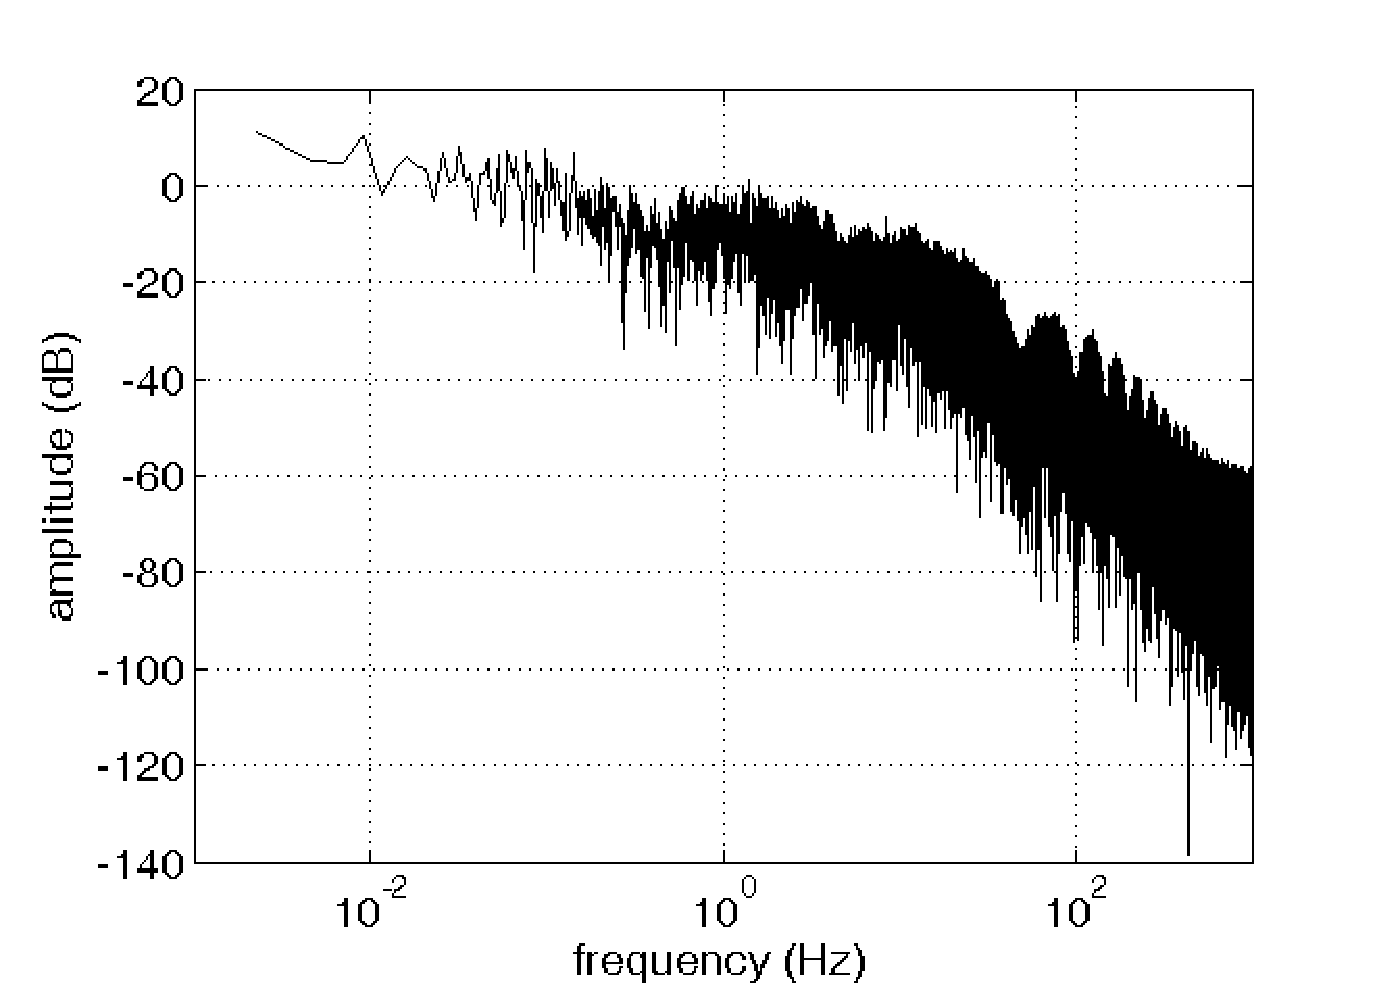
\includegraphics[width=0.3\textwidth]{spectrum_RMS0040.eps} &
    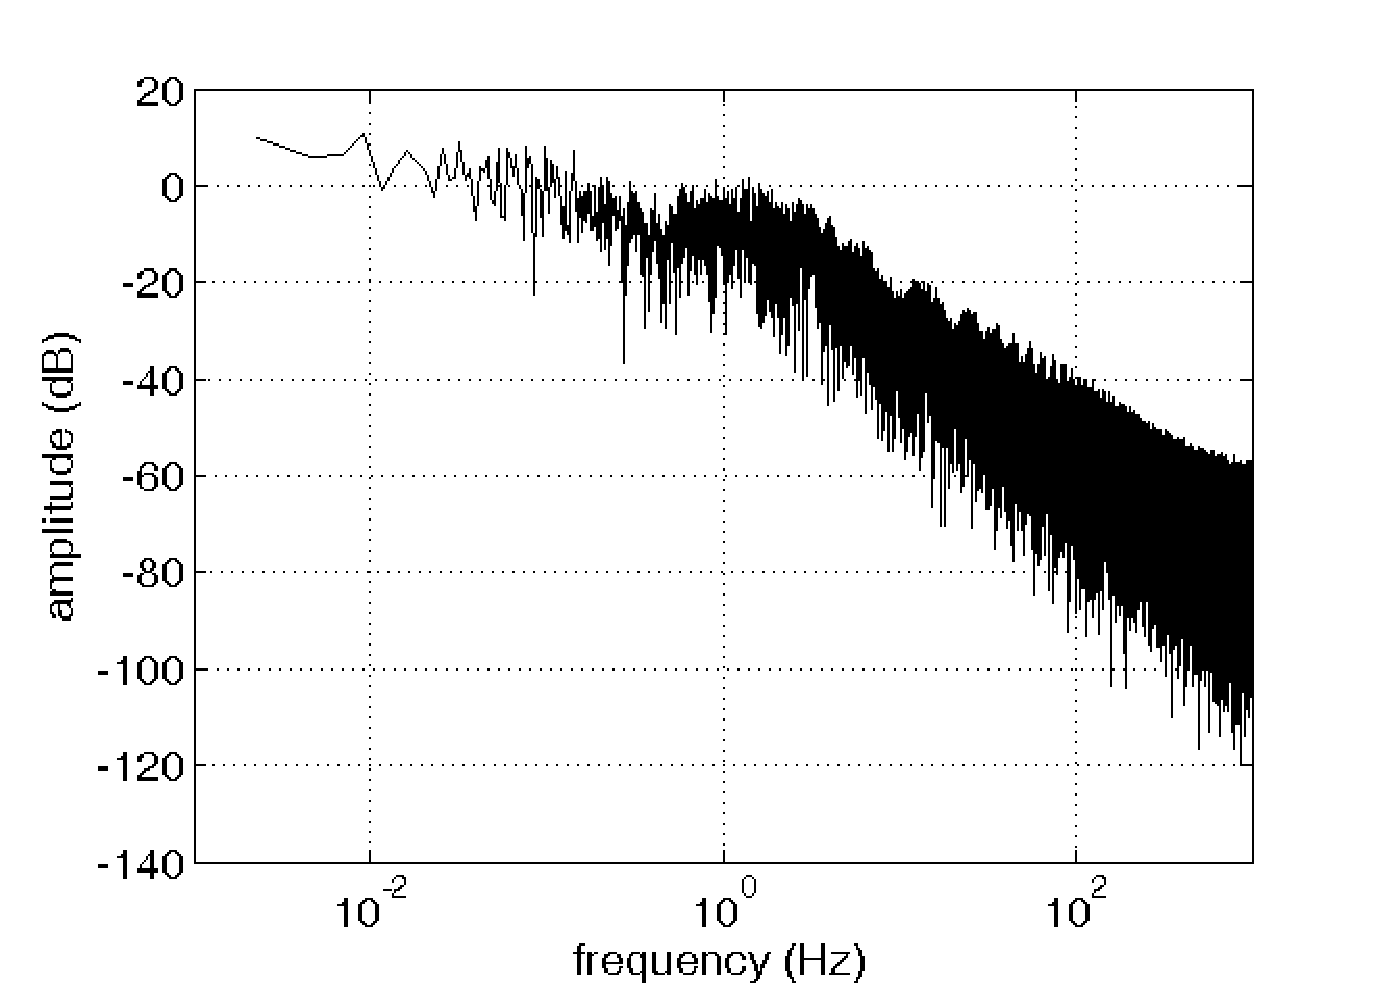
\includegraphics[width=0.3\textwidth]{spectrum_RMS0200.eps} &
    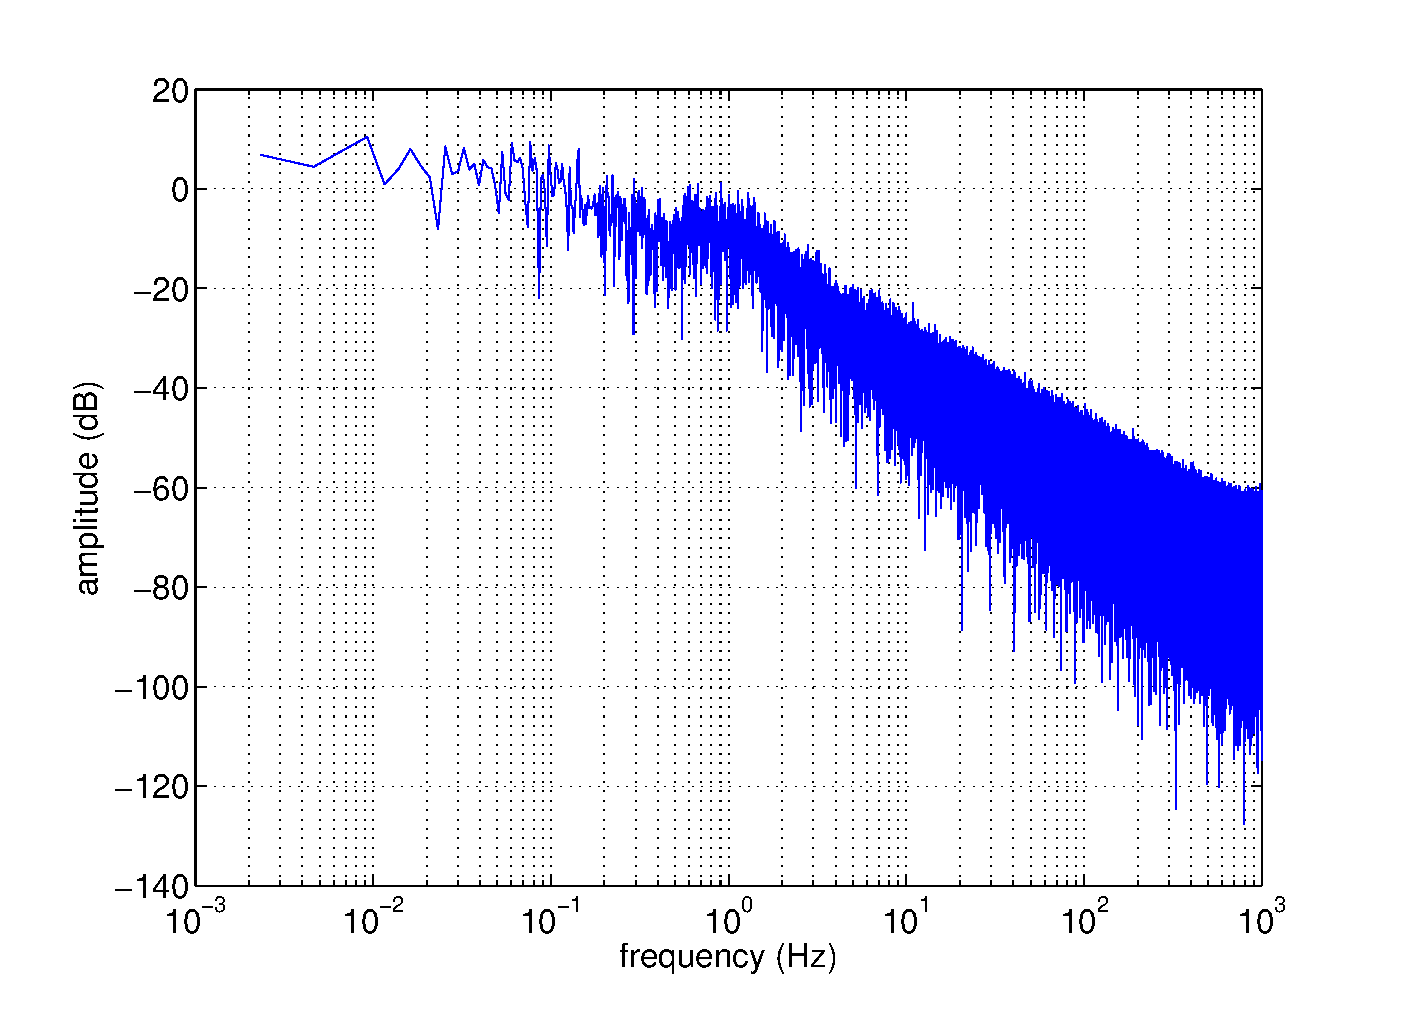
\includegraphics[width=0.3\textwidth]{spectrum_RMS1000.eps} \\
    $(a)$ & $(b)$ & $(c)$ \\
  \end{tabular}
%  \caption{(left to right) effects of the RMS on the bandwidth of the EMG
%    signals, for $T_{RMS} = 20, 100, 500ms$.}
%  \label{fig:RMSs}
\end{figure}

\newpage

\begin{figure}[!ht] \centering
  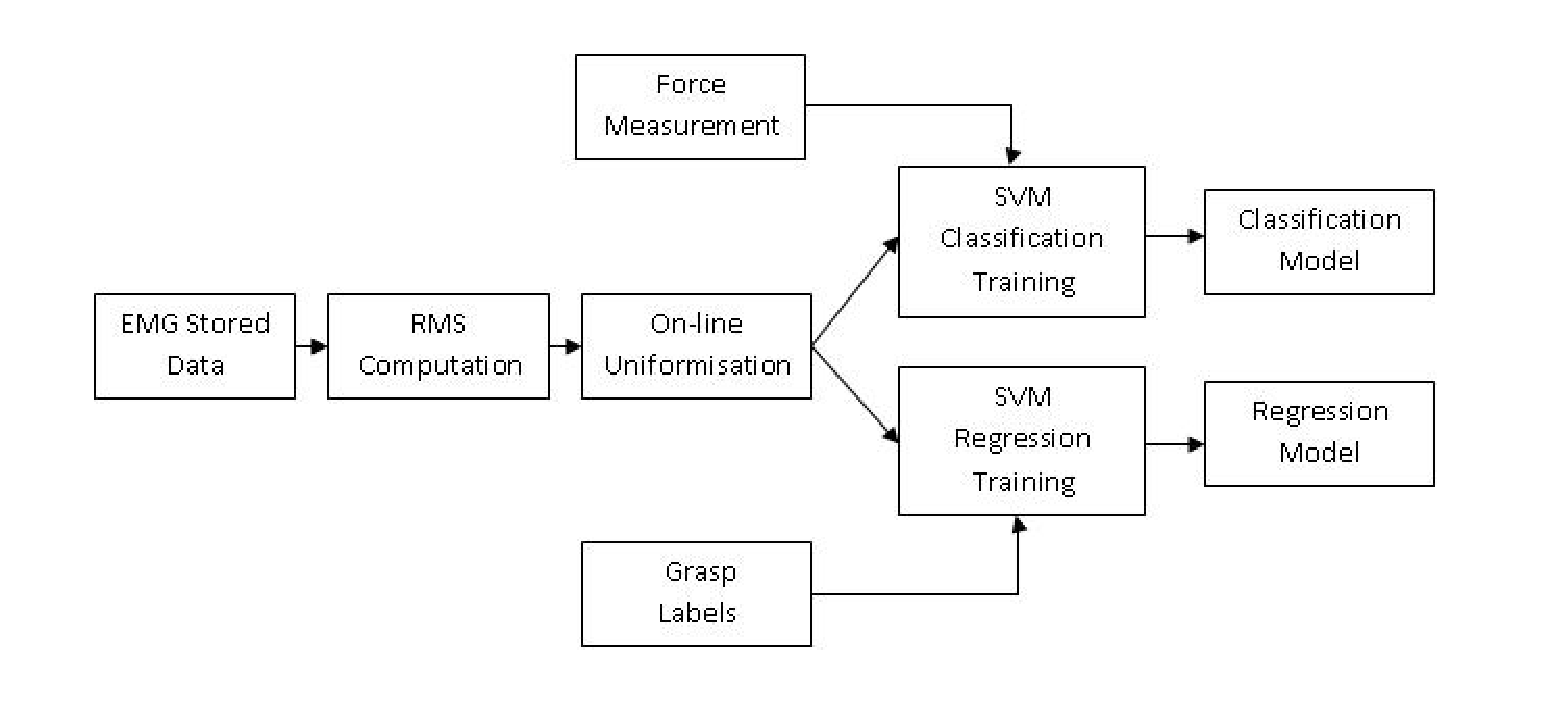
\includegraphics[width=0.75\textwidth]{Schema.eps} \\
%  \caption{Graphical representation of the system employed to solve our problem.}
%  \label{fig:Algorithm}
\end{figure}

\newpage

\begin{figure}[!ht] \centering
  \begin{tabular}{cc}
    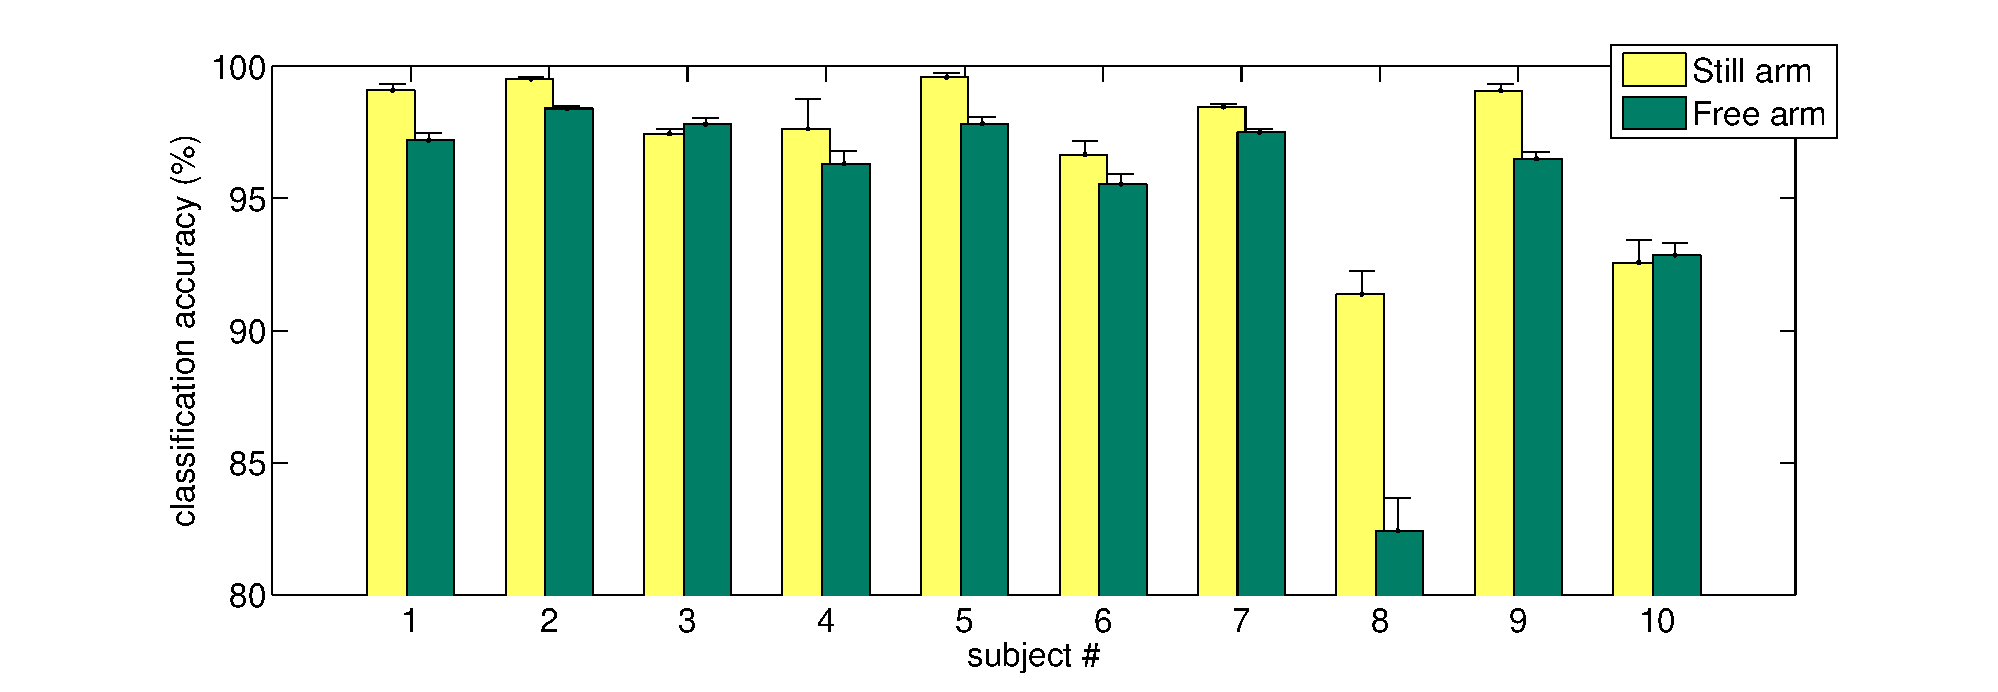
\includegraphics[width=0.45\textwidth]{perfClass.eps} &
    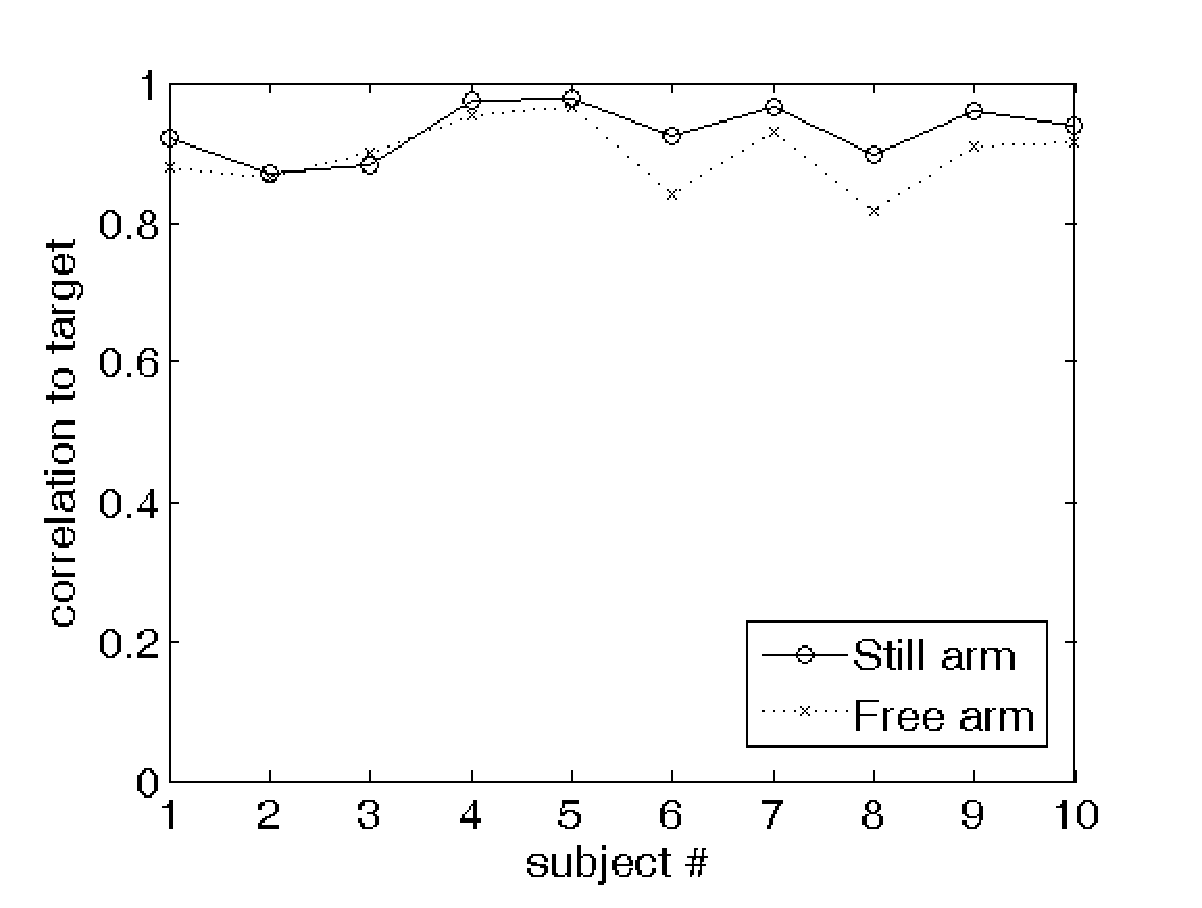
\includegraphics[width=0.45\textwidth]{perfRegr.eps} \\
    $(a)$ & $(b)$ \\
  \end{tabular}
%  \caption{classification $(a)$ and regression $(b)$ results obtained
%    by the system, on both phases of the experiment (FA and SA) and
%    for each subject.}
%  \label{fig:results}
\end{figure}

\newpage

\begin{figure}[!ht] \centering
  \begin{tabular}{cc}
    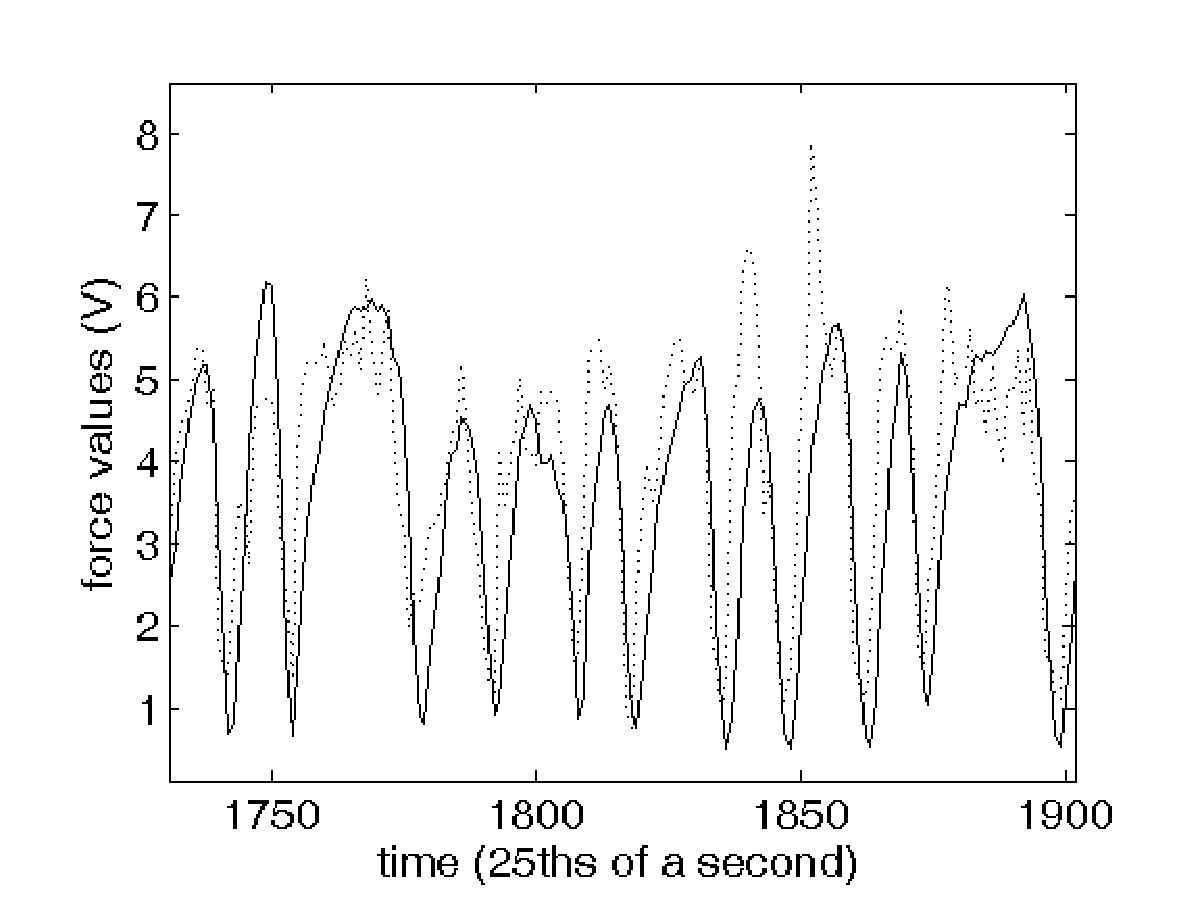
\includegraphics[width=0.45\textwidth]{example_6_one.eps} &
    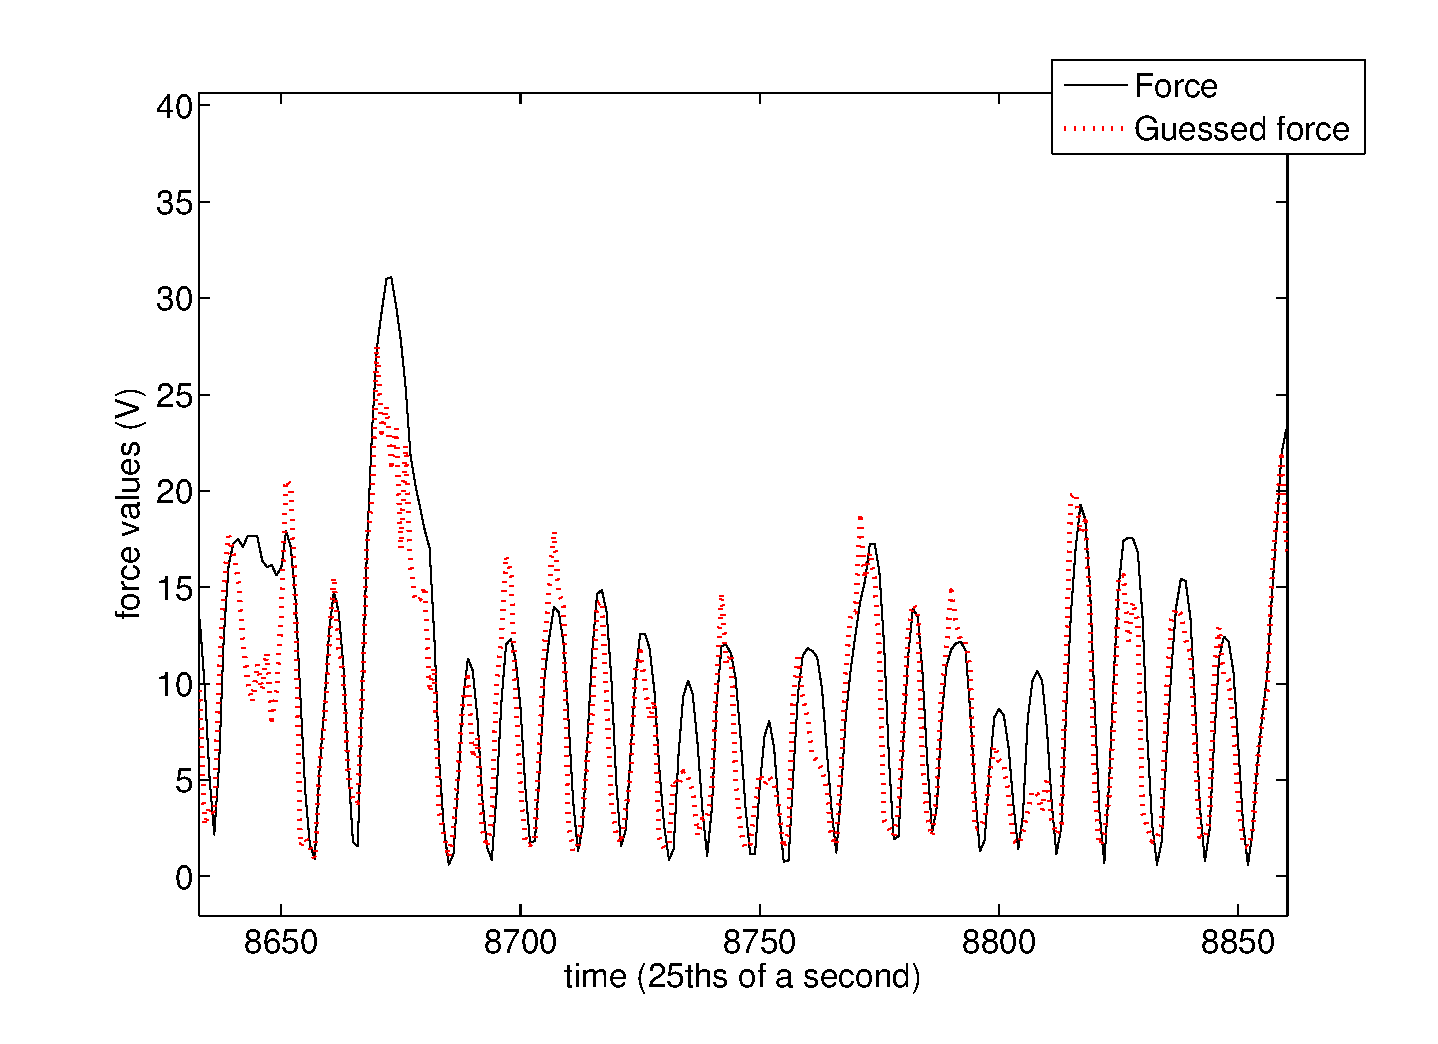
\includegraphics[width=0.45\textwidth]{example_6_two.eps} \\
    $(a)$ & $(b)$ \\
  \end{tabular}
%  \caption{comparing true (continuous line) and guessed (dotted line) force values for regression of a
%    typical subject (number $6$, FA phase).}
%  \label{fig:examples}
\end{figure}

\newpage

\begin{figure}[!ht] \centering
  \begin{tabular}{cc}
    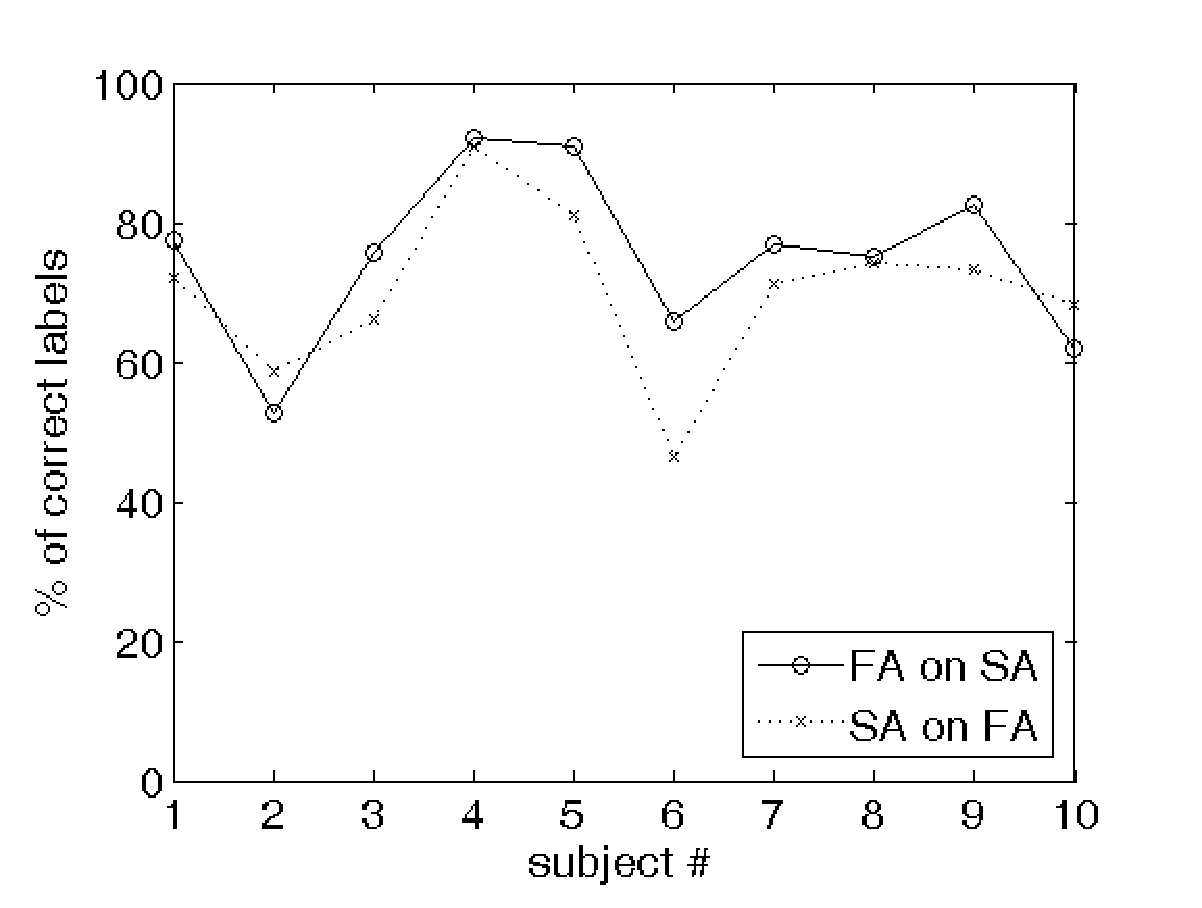
\includegraphics[width=0.45\textwidth]{2on1_class.eps} &
    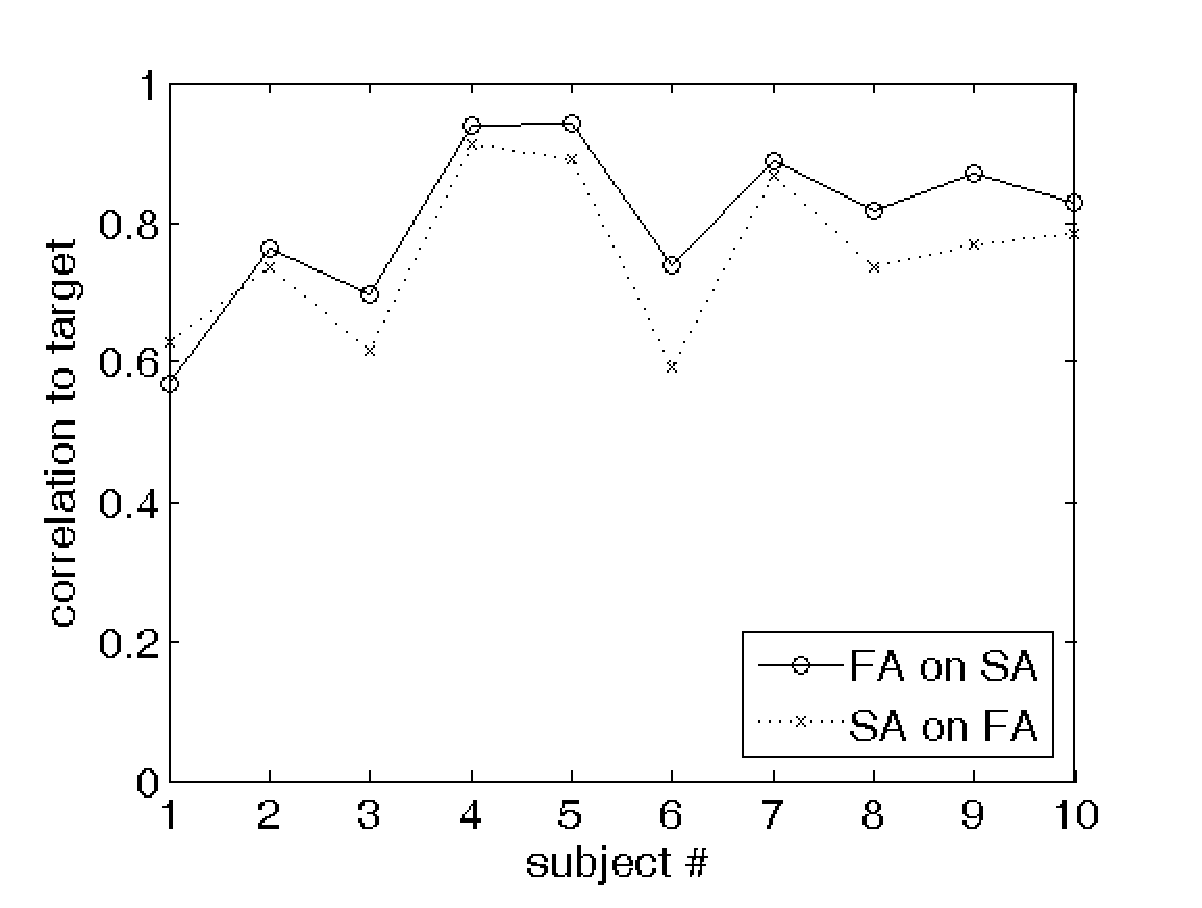
\includegraphics[width=0.45\textwidth]{2on1_regr.eps} \\
    $(a)$ & $(b)$ \\
  \end{tabular}
%  \caption{classification $(a)$ and regression $(b)$ results obtained
%    testing on SA-data models trained on FA, and vice-versa.}
%  \label{fig:2on1}
\end{figure}

\newpage

\begin{figure}[!ht] \centering
  \begin{tabular}{c}
    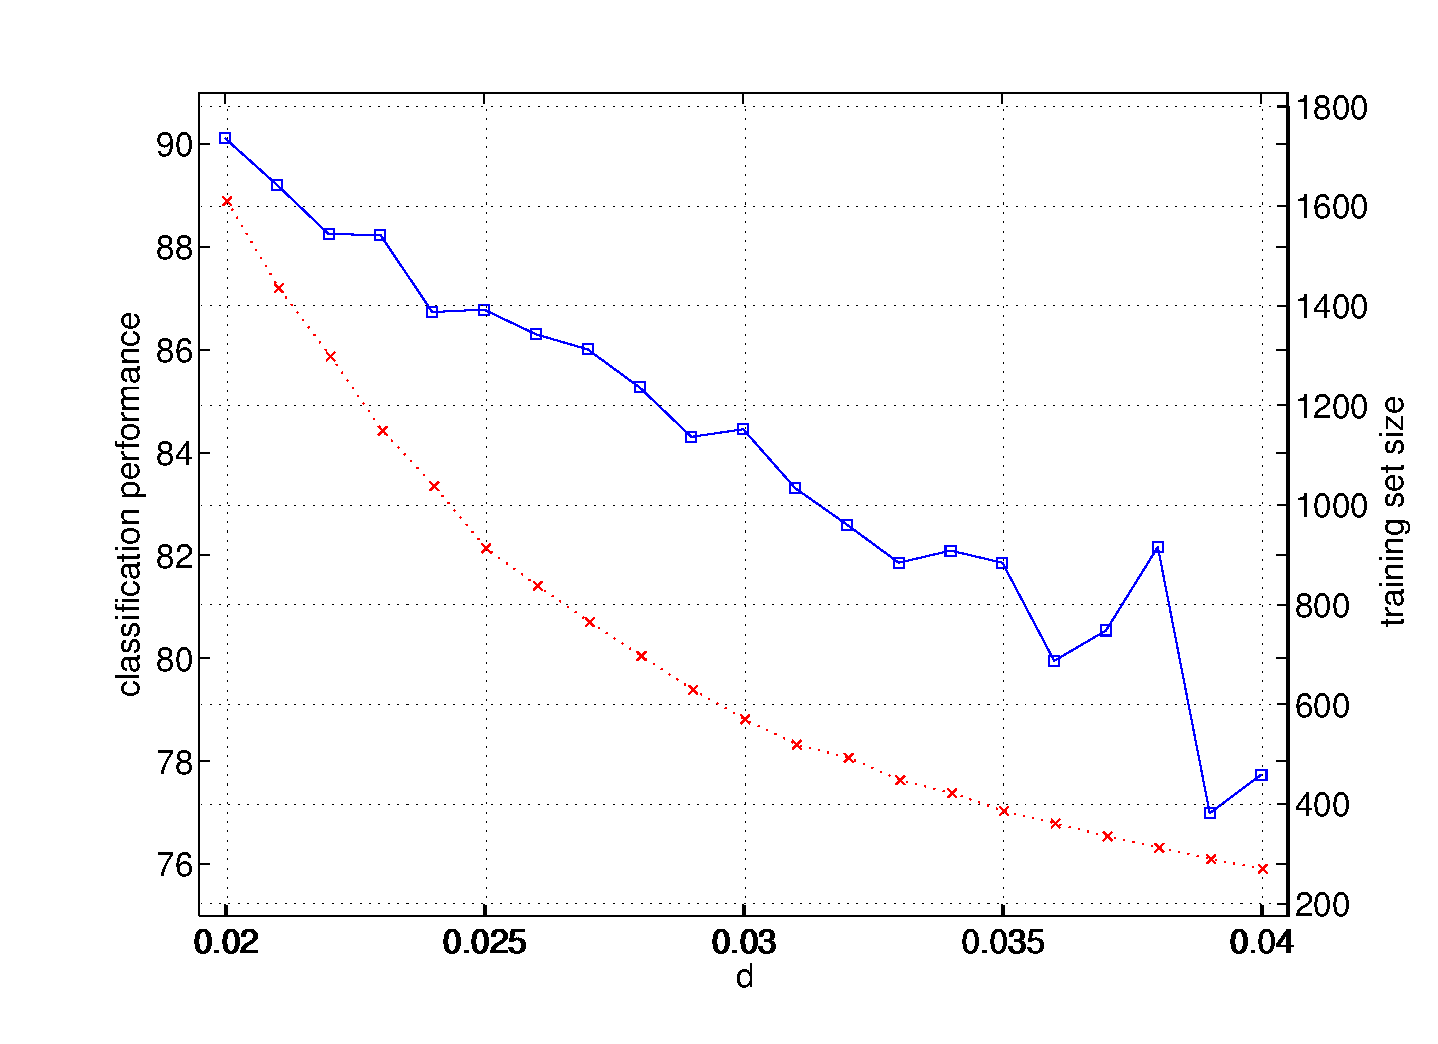
\includegraphics[width=0.6\textwidth]{subj8.eps} \\
  \end{tabular}
%  \caption{size of the training set (dotted line) and classification
%    performance (continuous line), of subject $8$ in the FA phase, as
%    $d$ changes.}
%  \label{fig:subj8}
\end{figure}

\newpage

\begin{figure}[!ht] \centering
  \begin{tabular}{cc}
    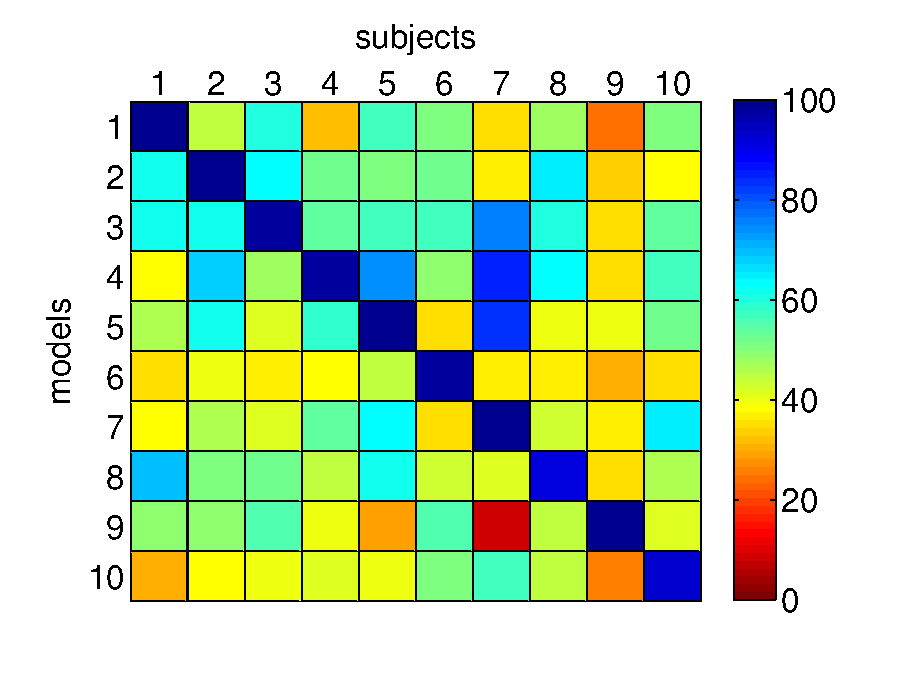
\includegraphics[width=0.45\textwidth]{crossClass1.eps} & 
    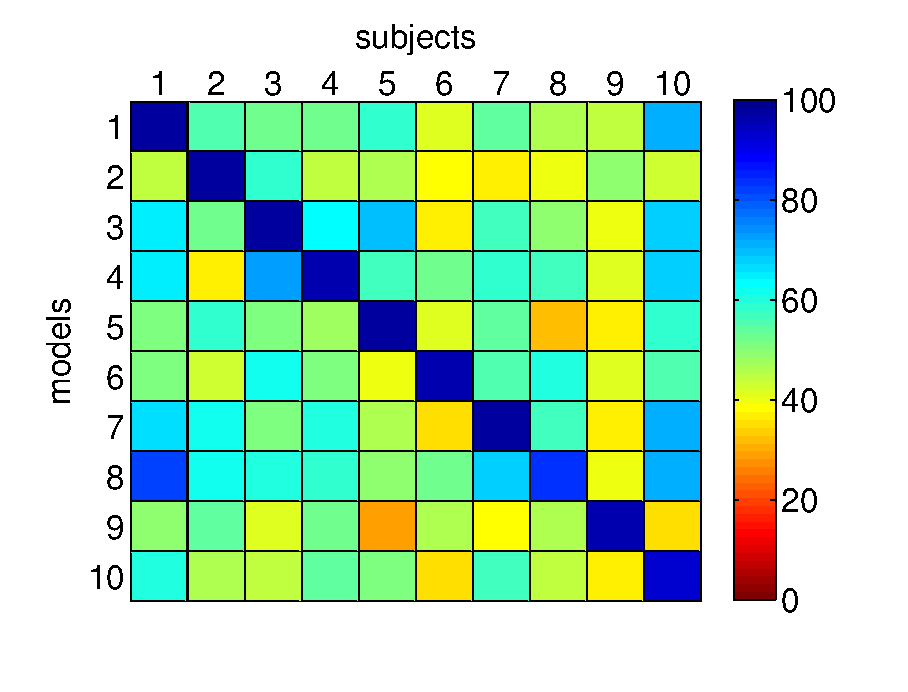
\includegraphics[width=0.45\textwidth]{crossClass2.eps} \\
    $51.69\% \pm 19.27\%$ & $54.04\% \pm 16.42\%$ \\
    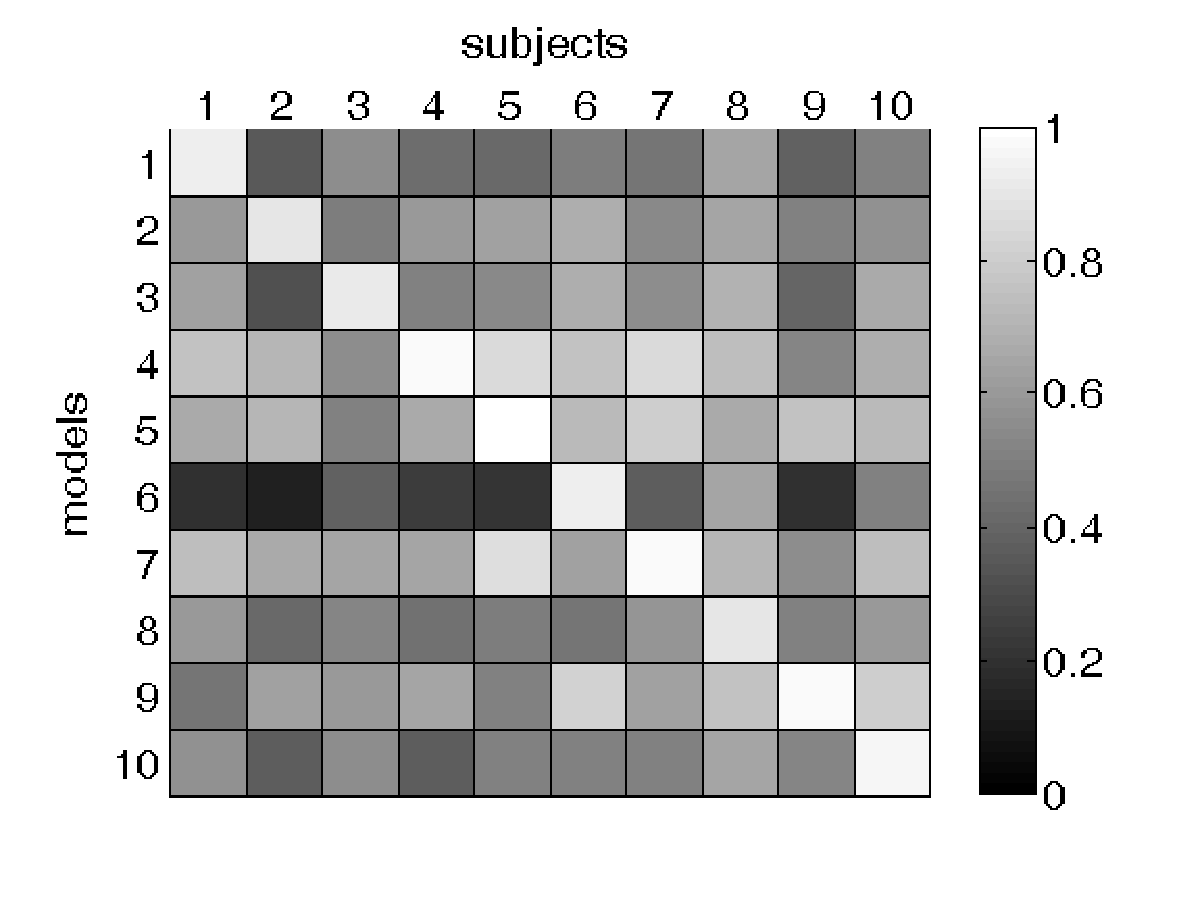
\includegraphics[width=0.45\textwidth]{crossRegr1.eps} & 
    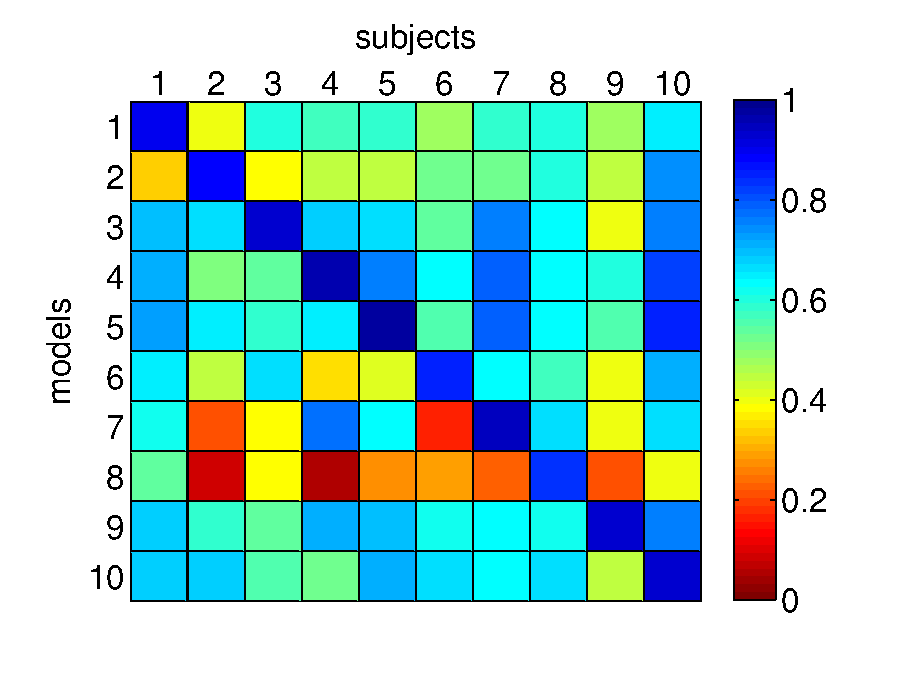
\includegraphics[width=0.45\textwidth]{crossRegr2.eps} \\
    $0.60 \pm 0.18$ & $0.58 \pm 0.19$ \\
  \end{tabular}
%  \caption{cross-subject performance matrices, for classification (top
%    row) and regression (bottom row), in the SA (left column)
%    and FA phase (right column); the numbers refer to all element of
%    the matrices, excluding the diagonals.}
%  \label{fig:cross}
\end{figure}

\end(document)
